\section{Evaluation}
\label{sec:evaluation}

% Results figures, rendered from the persisted artifacts:
% bootstrap_ci.json (suite means and 95% CIs), stability_run1_vs_run2.json (run pairs).
% Values resolve through figures/generated_values.tex, which scripts/gen_sp_figures.py
% writes from those artifacts; run `python scripts/gen_sp_figures.py --check` to prove
% this figure still agrees with them.
% Layout discipline: the top panel shows point estimates + intervals only
% (no filled bars under the whiskers), the bottom panel's legend lives
% below the axis (never over the bars), and both panels share the same
% value range so the stacked scales read as one.
% GENERATED by scripts/gen_sp_figures.py -- do not edit by hand.
% Every plotted number in the S&P figures resolves through this file, so a
% figure cannot silently disagree with the artifact it claims to show.
% Regenerate:  python scripts/gen_sp_figures.py
% Verify:      python scripts/gen_sp_figures.py --check
% Sources:
%   results/bootstrap_ci.json
%   results/stability_run1_vs_run2.json
%   results/b4_baseline_zodiac_20260922.json
%   results/model_quality/chrollo_calibration.json
%   results/sp2027_rescue/behavior_trajectory_benchmark.json

\def\RaginLiveTechnique{0.9598}
\def\RaginLiveTechniqueErrLo{0.0122}
\def\RaginLiveTechniqueErrHi{0.0122}
\def\RaginLiveActor{0.8500}
\def\RaginLiveActorErrLo{0.0000}
\def\RaginLiveActorErrHi{0.0000}
\def\RaginLivePersona{0.7325}
\def\RaginLivePersonaErrLo{0.0587}
\def\RaginLivePersonaErrHi{0.0558}
\def\RaginLiveComposite{0.8796}
\def\RaginLiveCompositeErrLo{0.0224}
\def\RaginLiveCompositeErrHi{0.0204}
\def\RaginLivePersonaRunTwo{0.7504}
\def\RaginLiveCompositeRunTwo{0.8845}
\def\RaginPersonaRunDelta{0.018}
\def\RaginTechDelta{0.317}
\def\RaginTechDeltaLo{0.162}
\def\RaginTechDeltaHi{0.480}
\def\RaginActorDelta{0.140}
\def\RaginActorDeltaLo{0.083}
\def\RaginActorDeltaHi{0.197}
\def\RaginPersonaNullDelta{0.005}
\def\RaginPersonaNullDeltaLo{-0.047}
\def\RaginPersonaNullDeltaHi{0.057}
\def\RaginOverallDelta{0.154}
\def\RaginOverallDeltaLo{0.092}
\def\RaginOverallDeltaHi{0.221}
\def\RaginGroundingTtpCount{35}
\def\RaginNoGroundingTtpCount{0}
\def\RaginRoutingBefore{0.8875}
\def\RaginRoutingAfter{0.955}

\begin{figure}[t]
\centering
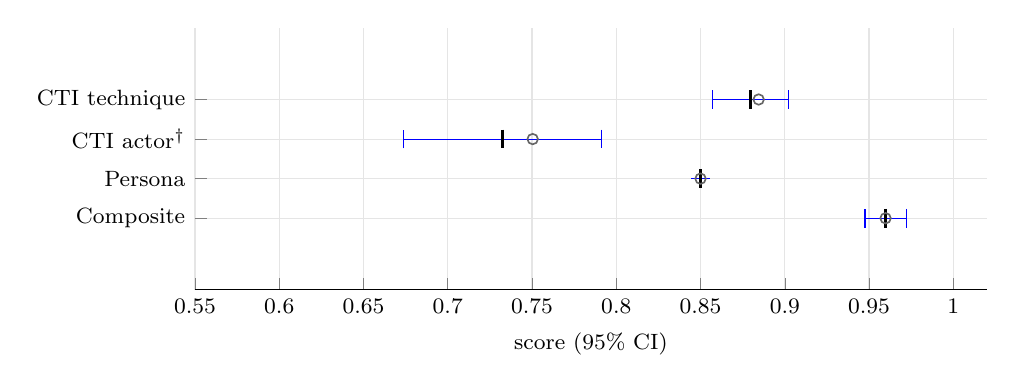
\begin{tikzpicture}
\begin{axis}[
  name=ax1,
  width=0.96\linewidth,
  height=4.9cm,
  xmin=0.55, xmax=1.02,
  y axis line style={draw=none},
  axis x line*=bottom,
  axis y line*=left,
  ytick=data,
  yticklabels={Composite,Persona,CTI actor$^{\dagger}$,CTI technique},
  y dir=reverse,
  xlabel={score (95\% CI)},
  xlabel style={font=\footnotesize},
  tick label style={font=\footnotesize},
  enlarge y limits=0.6,
  grid=major,
  grid style={black!10},
  clip=false
]
% point estimates and bootstrap 95% CIs from bootstrap_ci.json;
% only marks + intervals: no bars beneath the whiskers
\addplot+[only marks, mark=|, mark size=3.4, mark options={thick,black},
  error bars/.cd, x dir=both, x explicit] coordinates {
  (\RaginLiveTechnique,3) +- (\RaginLiveTechniqueErrLo,\RaginLiveTechniqueErrHi)
  (\RaginLiveActor,2) +- (\RaginLiveActorErrLo,\RaginLiveActorErrHi)
  (\RaginLivePersona,1) +- (\RaginLivePersonaErrLo,\RaginLivePersonaErrHi)
  (\RaginLiveComposite,0) +- (\RaginLiveCompositeErrLo,\RaginLiveCompositeErrHi)
};
% run-2 overlay: open markers (point estimates from stability_run1_vs_run2.json;
% per-suite CIs were not computed for run 2, so none are drawn)
\addplot+[only marks, mark=o, mark size=1.9, mark options={semithick,black!60}] coordinates {
  (\RaginLiveTechnique,3)
  (\RaginLiveActor,2)
  (\RaginLivePersonaRunTwo,1)
  (\RaginLiveCompositeRunTwo,0)
};
\end{axis}
\end{tikzpicture}

\vspace{2mm}

\begin{tikzpicture}
\begin{axis}[
  name=ax2,
  width=0.96\linewidth,
  height=4.9cm,
  ybar=1.5pt,
  bar width=9pt,
  ymin=0.55, ymax=1.0,
  symbolic x coords={CTI technique,CTI actor,Persona,Composite},
  xtick=data,
  ylabel={mean score},
  ylabel style={font=\footnotesize},
  tick label style={font=\footnotesize},
  ymajorgrids,
  grid style={black!10},
  enlarge x limits=0.25,
  legend style={font=\scriptsize, at={(0.5,-0.16)}, anchor=north, legend columns=2, draw=none, fill=none},
  legend cell align={left},
]
% run 1 vs run 2 from stability_run1_vs_run2.json
\addplot+[black!35, fill=black!35] coordinates {
  (CTI technique,\RaginLiveTechnique) (CTI actor,\RaginLiveActor) (Persona,\RaginLivePersona) (Composite,\RaginLiveComposite)
};
\addplot+[black!70, fill=black!70, pattern=north east lines] coordinates {
  (CTI technique,\RaginLiveTechnique) (CTI actor,\RaginLiveActor) (Persona,\RaginLivePersonaRunTwo) (Composite,\RaginLiveCompositeRunTwo)
};
\legend{run 1, run 2}
\end{axis}
\end{tikzpicture}
\caption{Live-campaign results from the persisted artifacts (identical
deterministic-strata bars across runs are the finding, not a plotting
error). All four plotted values are the \emph{both-channel} operational
score of Table~\ref{tab:live}, which fuses the served-text and CTI-analysis
channels; they are not served-quality results, and the echo-guarded bounds
for the same rows are 0.479 technique and 0.243 actor.
\emph{Top:}
suite means with bootstrap 95\% confidence intervals; open markers mark
the independent second run's point estimates, and the actor interval is
degenerate ($^{\dagger}$) because the actor rubric assigns the same
score to every row, so uncertainty is carried by the Wilson pass-rate
interval instead (Table~\ref{tab:live}). \emph{Bottom:} two independent
218-query campaigns; the deterministic CTI strata replicate exactly and
only the LLM-judged persona stratum moves, by $+\RaginPersonaRunDelta$.}
\label{fig:results}
\end{figure}


The evaluation asks whether each mechanism the design introduces
contributes measurably. We organize it by the four research questions of
\S\ref{sec:intro}: the value of grounding (RQ1), consistency and safety
under adversarial interaction (RQ2), deception quality against human
evaluators (RQ3), and the escalation pricing of each intelligence rung
(RQ4), followed by run-to-run stability and threats to
validity. Every quantitative claim in this section is traceable to a
persisted artifact in the released benchmark suite; where an interval is
reported it is a bootstrap 95\% confidence interval computed over paired
rows.

\subsection{Experimental Setup}
\label{sec:setup}

\subsubsection{Testbed}
All experiments run on the production single-host deployment described in
\S\ref{sec:implementation} (2~vCPU, ${\sim}4$~GB RAM). Generative
components use two model families from one free-tier provider: a generator
for deception drafts and a judge model for evaluation, chosen from a
different family than the generator. The provider catalog and quota are
probed by a scheduled watcher; one catalog removal (a third model) and one
quota-exhaustion window occurred during the study, both logged by the
watcher and both handled by the fallback path of \S\ref{sec:fallback}.

\subsubsection{Workloads}
Three query suites exercise the loop end to end:
\emph{CTI-technique} (123 queries asking how specific \attck techniques
are abused, scored on grounded technique coverage),
\emph{CTI-actor} (35 queries on named threat-actor behavior, scored on
attribution quality), and \emph{persona-realism} (60 interactive sessions
driven by scripted attacker personas, scored by an LLM judge on
host-believability rubrics). Each suite runs through the full verified
loop with HITL auditing enabled. The scenario sets are fixed and released,
so every run below is a re-run of the same 218 sessions.

\subsubsection{Metrics}
Suite scores are normalized to $[0,1]$ with a per-scenario pass threshold;
composite is the row-weighted mean. For the ablation we report
paired-difference bootstrap CIs, pairing rows by scenario across arms. For
consistency we report contradiction rate over targeted re-queries. For
deception quality we report a 1--5 rubric consensus over three evaluator
personas, scored on five dimensions: \emph{deception realism} (would the
output pass as the claimed service), \emph{persona consistency} (does
content match the attacker's skill tier), \emph{TTP accuracy} (are the
extracted \attck mappings correct and complete), \emph{engagement} (does
the response invite continued interaction rather than dead-ending), and
\emph{artifact safety} (is served credential material registered canary
bait rather than leakage). Each evaluator also records a rationale per
dimension; these rationales are what located the harness defect and the
fiction contradiction reported below.

\subsection{RQ1: Does Grounding Change What the Honeypot Detects?}
\label{sec:rq1}

We run the full 30-scenario-per-suite workload twice through the live
loop: once with retrieval grounding enabled and once with Don bypassed
(prompts otherwise identical), pairing every scenario across arms. This
is a direct test of G1 under the paired design that answers the
circularity concern: the same corpus, the same prompts, only retrieval
removed.

\begin{table}[t]
\centering
\caption{Paired RAG-vs-no-RAG differential (180 paired rows; 95\%
bootstrap CIs). Persona realism is predicted to be retrieval-independent,
and is.}
\label{tab:b4}
\begin{tabular}{lccc}
\toprule
Suite & RAG & No-RAG & $\Delta$ (95\% CI) \\
\midrule
CTI technique & 0.950 & 0.633 & $+0.317$ $[+0.162, +0.480]$ \\
CTI actor     & 0.850 & 0.710 & $+0.140$ $[+0.083, +0.197]$ \\
Persona       & 0.833 & 0.828 & $+0.005$ $[-0.047, +0.057]$ \\
\midrule
Overall (90 pairs) & & & $+0.154$ $[+0.092, +0.221]$ \\
\bottomrule
\end{tabular}
\end{table}

Table~\ref{tab:b4} shows the result. Grounding lifts technique detection
by $+0.317$ and actor attribution by $+0.140$, both intervals excluding
zero. The mechanism claim is starker: the grounded arm detects 35 distinct
TTPs across the campaign; the ungrounded arm detects none. The persona
stratum is the informative null: its interval straddles zero, exactly as
the architecture predicts, because host-believability is produced by the
deception engine and the fiction graph, not by threat-intelligence
retrieval. An ablation that produced only wins would look manufactured;
this one discriminates. The mechanism claim is consistent at the
deployment level: the grounded arm passes 30 of 30 technique scenarios;
the ungrounded arm passes 22 of 30, failing precisely the
synthesis-shaped scenarios (multi-step technique chains, actor-conditioned
campaign context) where static templates have nothing to say.

\emph{Takeaway: grounding is responsible for the intelligence the system
produces, and the ablation localizes the effect to exactly the suites
that need it.}

\subsection{RQ2: Consistency and Safety Under Adversarial Interaction}
\label{sec:rq2}

\subsubsection{Fiction-graph consistency}
We re-query 45 facts across live sessions (kernel versions, hostnames,
listening services, database engines, credentials) using adversarial
phrasings designed to induce drift, then compare each response against
the session's fiction graph. The graph-full configuration serves zero
contradictions across 45 re-queries (95\% CI upper bound $0.079$, i.e.,
the true contradiction rate is below 8\% even at the interval's
pessimistic edge), replays byte-identically, records
zero pinned-identity violations, and serves no response after a failed
verification verdict. The no-enforcement baseline provides none of these
properties (verifier coverage 45/45 turns versus 0). One failure this
benchmark caught during development is instructive: a benign
\texttt{uname} re-query was briefly flagged as a contradiction because
the extraction layer matched a distribution alias against the pinned
kernel string, a false contradiction we fixed and regression-locked; the
verifier now fails safe (unverifiable facts are rewritten or withheld,
never served on faith).

\subsubsection{Predictive steering}
The \attck predictor converts observed techniques into ranked next-move
candidates, and the deception plan attaches bait for the top candidates.
Across 10 predictions grounded in the session corpora, top-3 next-technique
accuracy is $0.9$, top-1 is $0.5$ (against a kill-chain prior of
${\approx}0.4$ for single-label prediction), MRR is $0.667$, and the
steered bait reaches the plan in $0.9$ of sessions. The A2 ablation
confirms the bait signal comes from the steering context: removing it
collapses steer-to-plan from $0.9$ to $0.4$.

\subsubsection{Mechanism ablations}
\begin{table}[t]
\centering
\caption{Ablation battery over the eight ground-truth scenarios
(persisted audit counts). Each removed mechanism should cost the system
the property it was added to provide; A5 tests path equivalence, not
degradation.}
\label{tab:ablations}
\small
\setlength{\tabcolsep}{4pt}
\begin{tabular}{>{\raggedright\arraybackslash}p{2.4cm}>{\raggedright\arraybackslash}p{3.3cm}>{\raggedright\arraybackslash}p{1.9cm}}
\toprule
Configuration & Observable in audit & Cost \\
\midrule
full (reference) & 8/8 verified serves; strategy and & -- \\
 & fiction blocks in 8/8 plans; 3 gated & \\
A1 no fiction graph & fiction block in 0/8 plans & plan loses \\
 & & fact binding \\
A2 no bait steering & strategy block in 0/8 plans; & steer-to-plan \\
 & & $0.9 \to 0.4$ \\
A3 no verifier & 8/8 served with no verdict & zero verified \\
 & & serves \\
A4 no HITL gate & 3 require-class contents served & governance \\
 & ungated & lost \\
A5 no graph engine & 8/8 verified, same serves & none (equivalent) \\
\bottomrule
\end{tabular}
\end{table}
Table~\ref{tab:ablations} summarizes the battery. Each row removes one
mechanism and tests the goal from \S\ref{sec:goals} that motivated it;
all four degrade as designed, and the linear fallback
path is behaviorally equivalent when the graph adds no information (G4).

\subsubsection{Live campaign}
\begin{table}[t]
\centering
\caption{Live 218-query campaign (verified loop, per-row bootstrap CIs).
Zero errors; 218/218 sessions engaged; 218/218 correct persona
assignments; 132 TTPs (67 unique) detected with zero false-positive CTI
alerts. Serve-path provenance: 88.1\% verified-generation serves,
11.9\% vetted deterministic, zero fallback serves.}
\label{tab:live}
\begin{tabular}{lccc}
\toprule
Suite & $n$ & Mean & 95\% CI \\
\midrule
CTI technique & 123 & 0.960 & $[0.948, 0.972]$ \\
CTI actor     & 35  & 0.850 & $[0.850, 0.850]^\dagger$ \\
Persona       & 60  & 0.733 & $[0.674, 0.788]$ \\
\midrule
Composite     & 218 & 0.880 & $[0.857, 0.900]$ \\
\bottomrule
\multicolumn{4}{l}{\footnotesize $^\dagger$Degenerate by construction: the actor rubric assigns the} \\
\multicolumn{4}{l}{\footnotesize same composite to every row, so the mean's bootstrap} \\
\multicolumn{4}{l}{\footnotesize interval carries no width; pass-rate uncertainty is} \\
\multicolumn{4}{l}{\footnotesize reported instead (Wilson $[0.901, 1.0]$).} \\
\end{tabular}
\end{table}
Table~\ref{tab:live} reports the full campaign and
Figure~\ref{fig:results} (top) renders the suite means with their
intervals. The persona stratum is
the binding floor: 58 of 60 sessions pass, and the failures are
timeout-shaped turns under provider safety-alignment pressure rather
than deception failures, consistent with the provider-fragility
analysis of \S\ref{sec:discussion}.

\emph{Serve-path provenance.} Zero errors should not be read as the
deterministic path absorbing the campaign: a latency-split analysis of
the per-row serving times (\path{serve_provenance.json}) attributes
88.1\% of run 1's serves (87.2\% of run 2's) to the verified-generation
path -- an LLM draft admitted by the serving-time verifier -- and the
remaining 11.9\% / 12.8\% to vetted deterministic content (protocol
fast-paths, bait deployments). The split is suite-dependent: 100\% of
actor rows and 81--95\% of technique and persona rows served
LLM-verified, and the estimate is stable at a 2\,s threshold while
shifting only at 10\,s (threshold sensitivity is persisted). Decisively,
\emph{fallback serves are zero}: no row in either run records a failed
verifier verdict, so the fail-safe template swap never engaged -- the
vetted share is the loop's designed deterministic rung doing its job on
protocol-shaped turns, not degradation. The composite of Table~\ref{tab:live}
is therefore a measure of verified generative quality on roughly nine
serves in ten and of vetted deterministic content quality on the
remainder.

\emph{Auditing the persona judge.} Because the persona stratum's
automated judge is a deterministic realism rubric, it can be audited
exhaustively offline against the transcripts it scored -- a check the
LLM-as-a-judge literature recommends for learned judges
\cite{zheng2024}. Two systematic errors surfaced
(\path{live_benchmark_judge_panel_corrected.json}). First, \emph{bait
blindness}: on a credential-hunt query, the loop served registered
canary credentials -- the correct deception outcome under the
canary-registry construction of \S\ref{sec:design}, which bars real
secrets from the serving path -- and the rubric, which rewards realism
signals and penalizes brevity, scored the concise bait deployment
$0.25$. Second, \emph{harness contamination}: one row whose transcript
is a session-harness echo bug (the query re-emitted as a shell command,
then ``command not found'') entered the deception mean at $0.0$ despite
measuring nothing about deception. The audit re-scores both runs with
three corrections: reclassifying harness artifacts out of the deception
mean, applying the credential-bait floor ($0.85$) to rows that deploy
key-shaped canaries on credential-hunt queries, and rounding persisted
floats. The correction is small in aggregate -- persona means move
$0.733\to0.756$ and $0.750\to0.762$ -- but it is directional and it
removes a bias against the system's best behavior: the canary-bias
magnitude, the score mass the judge had moved against correct bait
deployments, is 1.35 points across the two runs. The rubric was patched
consistently (deployment floor applied after penalties), the audit
script and corrected judge carry regression tests, and both raw and
corrected means are released rather than silently substituted.

\emph{Takeaway: the consistency and safety properties hold under targeted
adversarial pressure, and each mechanism in the loop is individually
necessary.}

\subsection{RQ3: Deception Quality Against Human Evaluators}
\label{sec:rq3}

An LLM honeypot can be internally consistent and still be unconvincing,
so we score the end product. Eight ground-truth scenarios (credential
hunts, service enumeration, cloud-metadata probes, exfiltration staging)
are executed live and the full transcripts are scored on a 1--5 rubric
(deception realism, persona consistency, TTP accuracy, artifact safety)
by three evaluator personas. Consensus is the per-scenario mean across
evaluators; exact agreement across the three personas is $0.750$ -- a
within-model consistency figure, since all three personas share one
judge model (Appendix~\ref{app:rubrics}), not inter-annotator agreement
in the human-study sense. The consensus score is
$\mathbf{3.86/5}$, with all eight scenarios at or above 3, five of eight
at 4 or above, and the best scenario (service enumeration) at $4.20$.
Table~\ref{tab:consensus} gives the per-scenario consensus with the
rubric profile.

\begin{table}[t]
\centering
\caption{Per-scenario consensus (mean of three evaluator personas over
the 1--5 rubric). The rubric profile of the weakest scenario locates the
weakness in persona realism and artifact safety, not in the deception's
technique accuracy.}
\label{tab:consensus}
\small
\setlength{\tabcolsep}{3.5pt}
\begin{tabular}{lcccccc}
\toprule
Scenario & Decep. & Pers. & TTP & Eng. & Art. & Overall \\
\midrule
GT-001 whoami        & 4.0 & 4.0 & 5.0 & 4.0 & 3.7 & 4.1 \\
GT-002 show creds    & 4.0 & 4.0 & 5.0 & 4.0 & 4.0 & 4.2 \\
GT-003 privesc       & 4.0 & 3.7 & 5.0 & 4.0 & 3.3 & 4.0 \\
GT-004 IMDS/SSRF     & 4.0 & 4.0 & 4.3 & 4.0 & 3.3 & 3.9 \\
GT-005 SQLi          & 2.3 & 2.7 & 5.0 & 4.0 & 1.0 & 3.0 \\
GT-006 services      & 4.0 & 4.0 & 5.0 & 4.0 & 4.0 & 4.2 \\
GT-007 reverse shell & 3.0 & 3.0 & 3.0 & 4.0 & 4.0 & 3.4 \\
GT-008 shadow dump   & 4.0 & 4.0 & 4.7 & 4.3 & 3.7 & 4.1 \\
\midrule
\textbf{Consensus} & & & & & & \textbf{3.86} \\
\bottomrule
\end{tabular}
\end{table}

Three protocol details matter for interpreting the number. First,
evaluators score complete transcripts, not excerpts; an earlier scoring
pass on truncated transcripts depressed two scenarios by up to $0.8$ and
was rerun after we fixed the harness. Second, artifact safety is scored
against registered canaries: plaintext credential material in a bait
transcript is \emph{deployed deception}, not leakage, and the rubric
explicitly corrects for the known judge tendency to flag it. Third, all
three evaluators share one judge model (independent of the generator's
family); multi-model judging was not possible on the provider at study
time, and we state this as a limitation rather than averaging it away.

The weakest scenario ($3.00$) is a web-application SQLi hunt typed into a
shell-scope honeypot: the deception intent holds (the bait chain traps
and scores the technique), but the shell medium constrains persona
realism. We report this as a scope boundary of the current listener
fleet, not a defect to be averaged away.

\emph{Takeaway: the deception holds a three-evaluator consensus above the
acceptance bar on every scenario, with the failure modes named rather
than smoothed.}

\subsection{RQ4: Pricing the Ladder -- Adaptive Kind-Awareness and Its
Fold-Down}
\label{sec:jeveval}

The top rung of the ladder (\S\ref{sec:ladder}) is adaptive: a
kind-aware assessment layer (\emph{Jev}) that reads session behavior and
returns the attack kind and skill tier that the routing and deception
layers should act on. We price it in three experiments, each with its
artifact released.

\emph{Assessment quality on real logs.} On 13 replayed sessions drawn
from real Cowrie logs, the baseline pipeline without kind-awareness
correctly assessed 0; with it, 12 of 13
(\path{jev_real_logs_eval.json}). The one miss was a session whose
recorded behavior was consistent with two kinds; we report the miss
rather than resolve it by hindsight.

\emph{Steering effect.} A 200-session stratified A/B on routing decisions
(50 per skill tier, \path{jev_ab_eval.json}) shows the ladder's descent
in action. In the first pipeline revision, kind-aware enrichment lifted
routing accuracy from 69.5\% to 91.5\%, fixing 44/44 misrouted APT
sessions with zero regressions. The final revision then reproduced that
entire gain deterministically: an apt skill-map repair, a weighted
behavior-severity floor, and an n-gram-feature retrain of the classifier
(0.8875 $\to$ 0.9550) reach 100\% with the assessment layer contributing
zero marginal accuracy ($\Delta = 0.0$, $n=200$). Both arms sit at the
pass ceiling, so this comparison alone cannot separate ``the floor
already covers everything the assessment layer adds'' from ``the
benchmark contains nothing left to cover'': a routing decision is scored
correct when it meets the tier's risk floor, and the floor mechanism
meets it on every sampled session. We therefore census the full
400-session held-out corpus for the stratum where the comparison is
informative -- sessions whose deterministic routing lands below the tier
floor (\path{jev_hard_subset.json}). The stratum is small: six sessions,
all APT-tier, all exactly one rung under floor, drawn from the
classifier's lower-confidence tail (mean confidence 0.53 versus 0.75
corpus-wide). On this stratum the assessment layer was evaluated live:
one session was assessed and rescued (baseline \emph{high} $\to$
assessment \emph{critical} $\to$ final at floor); the remaining five
returned empty assessments after provider refusals -- the free-tier
endpoint refuses security-shaped payloads, a behavior a controlled
probe confirmed (benign command states serve; attacker-tooling states
receive HTTP 403). A structured retry measurement (four attempts per
row, spaced) recovered none of the five, and the refusal pattern
varied across executions -- the rescue itself appears to have been a
transient pass rather than a stable availability mode. The top rung's marginal
effect on routing is therefore unmeasured in both directions, for two
compounding reasons: informative sessions are rare under the current
floor, and they are exactly the sessions the provider is least willing
to assess. The removal stands on its measured record -- zero marginal
effect on every row the benchmark resolves, zero regression risk added
by removal, and a provider dependency eliminated -- but the bound is
stated rather than claimed away: the result is \emph{no measurable
marginal effect at this benchmark's resolution}, not general subsumption.
Table~\ref{tab:hardsunset} summarizes the census and the live arm.
The availability result strengthens the removal on its own terms: a
rung that returns empty precisely on APT-shaped sessions is a liability
on the highest-stakes traffic, independent of what its accuracy would
be when it answers.

\begin{table}[t]
\centering
\caption{Fold-down hard-subset census (the released
\texttt{jev\_hard\_subset.json}). The informative stratum for the routing
comparison is the set of held-out sessions whose deterministic routing
lands below the tier's risk floor; on every other row the assessment
layer cannot change the pass decision by construction. The live arm
assessed one of six informative sessions; the other five were refused
by the provider and did not recover on a structured retry protocol
(see text).}
\label{tab:hardsunset}
\small
\setlength{\tabcolsep}{4pt}
\begin{tabular}{@{}lc@{}}
\toprule
Census over the full held-out corpus & \\
(400 sessions) & \\
\midrule
Floor at or above tier floor & 394 \\
Informative (baseline below floor) & 6 \\
\quad tier & all APT \\
\quad under-floor depth & 1 rung \\
\quad classifier conf.\ (inf.\ / corpus) & 0.53 / 0.75 \\
\midrule
Live assessment arm (6 sessions) & \\
\midrule
Assessed and rescued (transient) & 1 \\
Unavailable; 0/5 recovered on structured retry & 5 \\
\bottomrule
\end{tabular}
\end{table}

\emph{Deception effect in closed loop.} Paired closed-loop replays pit a
simulated LLM attacker against the deception engine with and without
kind-aware guidance (\path{jev_dwell_replay_llm_REPORT.md}; 97.8\%
LLM-backed gateway calls, verified by a canary echo probe after an
earlier run was found to have silently template-fallen back). Bait
markers surfaced to the attacker rose from 4 to 9 (+125\%) across the
five error-free family pairs. Dwell time did not move: 34 vs.\ 33 turns
in the clean paired comparison. The report's own mechanism analysis
explains the null: in both arms, nearly every early leave cites
inconsistent fictional filesystem state -- a cautious attacker reads
inconsistency as a trap signal, so response consistency, not deception
style, is the binding constraint. This is precisely why the fiction
graph and verifier sit below the adaptive layer in the ladder: the
consistency rungs are load-bearing for every rung above them.

\emph{Takeaway: the top rung buys assessment coverage and bait exposure,
not dwell time -- and its routing contribution, unresolvable at the
benchmark's ceiling and unavailable on the rows that matter most, was
compiled down to a deterministic floor. The clearest signal in this
evaluation about where intelligence belongs is also the one stated with
its resolution bound.}

\subsection{Run-to-Run Stability}
\label{sec:stability}

LLM-driven systems rarely report whether their numbers replicate, so we
ran the full 218-query campaign twice, independently, with identical
configuration (Figure~\ref{fig:results}, bottom). The composite moves
from $0.880$ to $0.884$ ($\Delta
+0.005$); per-row pass-decision agreement is $0.991$ (216 of 218 rows).
The deterministic strata reproduce exactly (technique and actor suites:
per-row mean absolute difference $0.000$); the persona stratum, the only
LLM-judged stratum, shows MAD $0.096$ with pass agreement $0.967$. The
headline metrics are identical across runs: 132 TTPs, 67 unique,
218/218 engagement, 218/218 persona assignment. This is the signature we
want: scored-deterministic claims reproduce deterministically, and the
only variance is bounded judge sampling noise.

Recomputed on the judge-audited rows of the previous subsection
(\path{stability_run1_vs_run2.json}, \path{audited_panel}), the
comparison is unchanged: the audited composite moves $0.883\to0.888$
($\Delta+0.005$) with the same $0.991$ pass agreement, and the audited
deception suite shows MAD $0.097$ with agreement $0.967$. Two facts are
worth recording. First, the run-to-run variance is generator-side: 32
of 60 persona rows differ between runs, only one of them touched by the
audit, so the MAD's variance comes from provider sampling, not judge
error. Second, the audited suite mean retains the reclassified harness
row at its recorded 0.0; the deception-only means excluding harness
artifacts -- $0.756$ and $0.762$ -- are persisted alongside it rather
than chosen silently.

\subsection{Threats to Validity}
\label{sec:threats}

\emph{Construct.} Suite scores reward grounded technique coverage; a
system could game them by keyword stuffing. The persona rubric and the
human consensus study exist partly to catch exactly that failure, and
the two agree. \emph{Internal.} The judge model shares a provider with
the generator (different family); the consensus protocol, rubric
corrections, and the deterministic strata bound but do not eliminate
provider-common-mode effects. \emph{External.} The deployment observes tailnet traffic only: no ambient internet background
radiation, no botnet churn, no real APT dwell time; the live fleet runs
one SSH listener plus HTTP and Telnet services on the same session
interface, so web-shaped attack surfaces in particular are
under-represented. The workload personas approximate
but do not replace live adversaries, and the consensus study's
evaluators, however adversarial, are models. \emph{Statistical.}
Bootstrap CIs are computed over paired rows; scenario counts per suite
(35--123) bound interval width, which we report rather than
over-claiming.
